\documentclass{article}

\usepackage[pctex32]{graphics}
\usepackage{amssymb}
\usepackage{amsmath}
\usepackage[left=3cm,top=2cm,right=3cm,nohead,nofoot]{geometry}
\usepackage{latexsym}
\usepackage{siunitx} 
\usepackage{epsfig}
\parindent0pt
\parskip6pt
\pagestyle{empty}
\usepackage[vskip=1em,font=itshape,leftmargin=3em,rightmargin=3em]{quoting}
\usepackage{framed}
\newenvironment{quotationb}%
{\begin{leftbar}\begin{quotation}\noindent}
{\end{quotation}\end{leftbar}}
\usepackage{pstcol}
\usepackage[shortlabels]{enumitem}
\newcommand{\R}{{\mathbb R}}
\newcommand*{\thead}[1]{\multicolumn{1}{c}{\bfseries #1}}
\newcommand{\norm}[2]{\left|\left| #2 \right|\right|_{#1}}
\title{Homework 1}
\author{Firstname Lastname}
\begin{document}
\maketitle
% Required for alignment

\sisetup{
  round-mode          = places, % Rounds numbers
  round-precision     = 3, % to 2 places
}

This is a small template for homework. 

\bigskip
{\Large {\bf Problem 1}}
\bigskip

\begin{quotationb}MNIST dataset is used for a classification tasks. Denote the dataset as $D = \left\{ x^{(i)}, y^{(i)}\right\}_{i=1}^{N}$, where $x^{(i)}$ is the image and $y^{(i)} \in \left\{0, 1, \dots, 9 \right\}$ is the groudtruth label. Let’s stretch the image into a one-dimensional vector (from $28 \times 28$ to $784 \times 1$) and transform the labels into one-hot vectors, e.g. $y^{(i)} = 2 \rightarrow  \begin{bmatrix}
0 & 0 & 1 & 0 & 0 & 0 & 0 & 0 & 0 & 0 \end{bmatrix}^T$. Your task is to derive the gradient, and implement the gradient descent (GD) algorithm to optimize the following linear regression problem:
$$
L\left( {\bf W} \right) = \frac{1}{N}\sum_{i=1}^{N} \norm{2}{{\bf W}x^{(i)} + {\bf w_0} - y^{(i)}}^2
$$
\noindent Here, ${\bf W}$ and ${\bf w_0}$ are the parameters of your linear model. Test different step sizes $\tau$ and discuss how it influences the result. Also, draw the curve of the training error and test error during optimization, and discuss how they evolve during optimization. You should program the algorithms by yourself. You are not allowed to use the predefined modules in PyTorch (e.g., \verb|nn.Linear|, \verb|optim.SGD|).
\end{quotationb}

First, we must derive an expression of the gradient. We note that the gradient is linear so:
$$
\nabla L({\bf W}) = \frac{1}{N} \sum_{i=1}^{N} \nabla \left( \norm{2}{{\bf W}x^{(i)} + {\bf w_0} - y^{(i)}}^2\right)
$$

The simplest way to evaluate this is to write the summand as the inner-product of a vector with itself:
$$
\begin{aligned}
\norm{2}{{\bf W}x^{(i)} + {\bf w_0} - y^{(i)}}^2 & = \left({\bf W}x^{(i)} + {\bf w_0} - y^{(i)}\right)^{T} \left({\bf W}x^{(i)} + {\bf w_0} - y^{(i)}\right)
\end{aligned}
$$
Distributing this multiplication and, once again, utilizing the fact that the gradient is a linear operator, we may quickly compute the gradient with respect to the parameters ${\bf W}$ and ${\bf w}_0$:

$$
\begin{aligned}
\nabla_{\bf W} \left({\bf W}x^{(i)} + {\bf w_0} - y^{(i)}\right)^{T} \left({\bf W}x^{(i)} + {\bf w_0} - y^{(i)}\right) & = 2\left({\bf W}x^{(i)} + {\bf w_0} - y^{(i)}\right) \left(x^{(i)}\right)^T\\
\nabla_{{\bf w}_0} \left({\bf W}x^{(i)} + {\bf w_0} - y^{(i)}\right)^{T} \left({\bf W}x^{(i)} + {\bf w_0} - y^{(i)}\right) & = 2 \left({\bf W}x^{(i)} + {\bf w_0} - y^{(i)}\right)
\end{aligned}
$$

Thus at each time step, we increment the parameters negatively in this direction with scaling provided by our choice of $\tau$. 


\begin{figure}[h!]
\centerline{
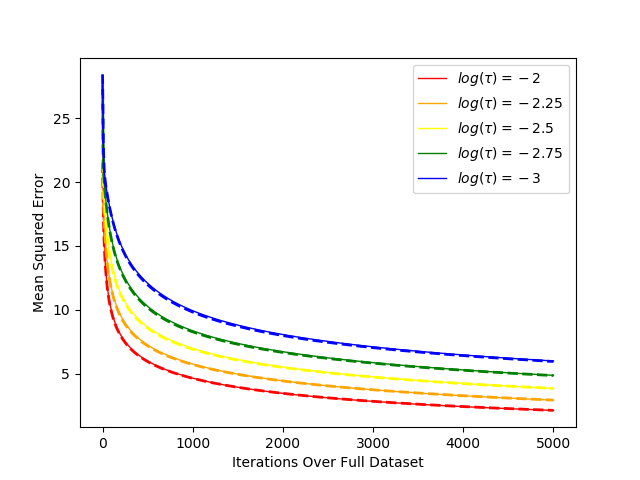
\includegraphics[width= 18cm]{img/problem_1/step_size.png}
}
\caption{\label{fig:fig1}Comparison of gradient descent method for various learning rates. Solid lines indicate mean squared error on the training data, and dashed lines indicate MSE on the test data.}
\end{figure}

\newpage

\bigskip
{\Large {\bf Problem 2}}
\bigskip

\begin{quotationb}Optimize the linear regression problem with Stochastic Gradient Descent (SGD). 
\begin{enumerate}[(a)]
\item Fixing the batch size $m$, test different step sizes $\tau$, draw the curves of training error and testing error, and discuss the influence of step size. 
\item Fixing the step size, test different batch sizes, draw the curves of training and testing error, discuss the influence of batch size
\item Use the same step size for GD and SGD. Draw the curves of training and testing error for both algorithms, where the $x$-axis is the number of training images used. Discuss the difference between both algorithms.
\end{enumerate}
\end{quotationb}

scooby


\begin{figure}[h!]
\centerline{
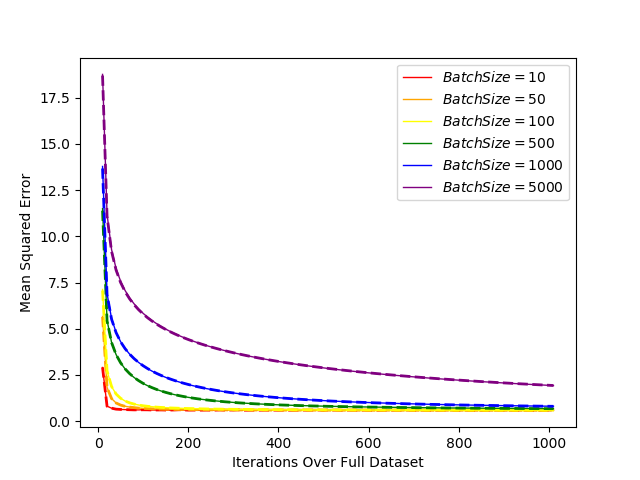
\includegraphics[width= 18cm]{img/problem_2/batch_comparison.png}
}
\caption{\label{fig:fig2}Comparison of stochastic gradient descent method for various batch sizes with a fixed learning rate of $\tau = 5e-3$. Solid lines indicate mean squared error on the training data, and dashed lines indicate MSE on the test data.}
\end{figure}

\begin{figure}[h!]
\centerline{
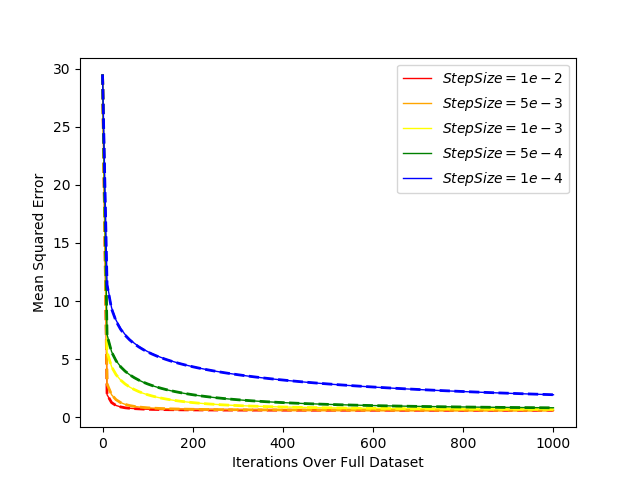
\includegraphics[width= 18cm]{img/problem_2/step_comparison.png}
}
\caption{\label{fig:fig3}Comparison of stochastic gradient descent method for various learning rates with a fixed batch size of 100. Solid lines indicate mean squared error on the training data, and dashed lines indicate MSE on the test data.}
\end{figure}

\newpage

\bigskip
{\Large {\bf Problem 3}}
\bigskip

\begin{quotationb}Let's add $L2$ regularization to the optimization problem:
$$
L\left( {\bf W} \right) = \frac{1}{N}\sum_{i=1}^{N} \norm{2}{{\bf W}x^{(i)} + {\bf w_0} - y^{(i)}}^2  + \lambda \left( a  \norm{F}{\textbf{W}}^2 + \norm{2}{\textbf{w}_0}^2 \right)
$$
This problem is also called {\it ridge regression}.
\begin{enumerate}[(a)]
\item Optimize the problem with SGD when $\lambda = 1$. Draw the curve of training and testing error
\item With $\lambda \in \left\{0.01, 0.1, 1, 10\right\}$, test how different choices of $\lambda$ influence the final test error.
\item Choose several hyperparameters with numbers you like, and use cross-validation to choose the best combination of $\lambda$, $\tau$, and $m$.
\end{enumerate}
\end{quotationb}

asld;kfja;lskdfj


\bigskip
{\Large {\bf Problem 4}}
\bigskip

\begin{quotationb}Let's move from fixed step size to changing step size. Use the best combination you obtained from the previous task. For the optimization problem in Problem 3, implement and report hte performance of
\begin{enumerate}[(a)]
\item decreasing step size
\item cosine step size scheduler
\end{enumerate}
with SGD. The cosine step size scheduler decays the step size with a cosine annealing for each iteration. Its expression is as follows:
$$
\tau_i = \gamma^i \left( \tau_{min} + \frac{1}{2} \left(\tau_{max} - \tau_{min}\right)\left(1 + \cos\left(\pi i / T \right) \right) \right)
$$
where $\tau_{min}$ and $\tau_{max}$ are ranges for the learning rate, and $T$ controls the period of the step size cyle. An annealing factor $\gamma$ is adopted to ensure the step size approaches zero. Compare and discuss the performance between (a), (b), and constant step size. 
\end{quotationb}

asdfasdf

\begin{table}[h!]
  \begin{center}
    \label{tab:table1}
    \begin{tabular}{r|S|S|S} % <-- Changed to S here.
      \thead{Batch Size } & \thead{$\lambda$ } & \thead{$\tau$} & \thead{MSE}\\
      \hline
      30 & 0.01 & 0.01 & 0.5931\\\
      100 & 0.01 & 0.01 & 0.5849\\\
      30 & 0.01 & 0.001 & 0.5828\\\
      \textbf{100} & \textbf{0.010} & \textbf{0.001} & \textbf{0.5821}\\\
      30 & 0.1 & 0.01 & 0.6218\\\
      100 & 0.1 & 0.01 & 0.6157\\\
      30 & 0.1 & 0.001 & 0.6130\\\
      100 & 0.1 & 0.001 & 0.6126
    \end{tabular}
    \caption{Cross-validation Results}
  \end{center}
\end{table}




\begin{figure}[h!]
\centerline{
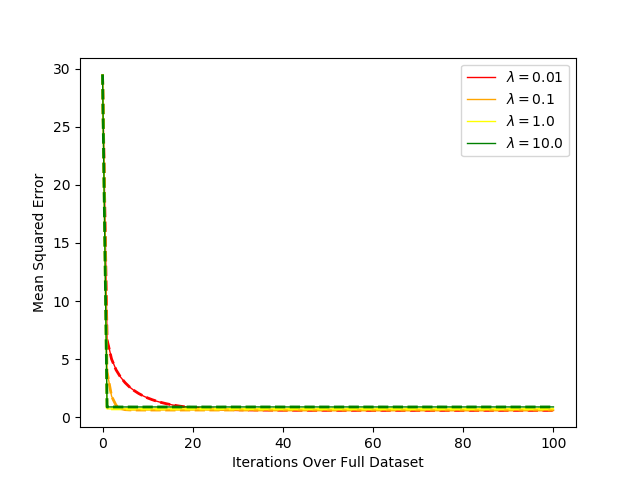
\includegraphics[width= 18cm]{img/problem_3/ridge_coeffs.png}
}
\caption{\label{fig:fig4}Comparison of stochastic gradient descent method applied to the ridge regression problem with various ridge coefficients. The batch size was fixed at 100, and the learning rate was fixed at $\tau=5e-3$. Solid lines indicate mean squared error on the training data, and dashed lines indicate MSE on the test data.}
\end{figure}

\begin{figure}[h!]
\centerline{
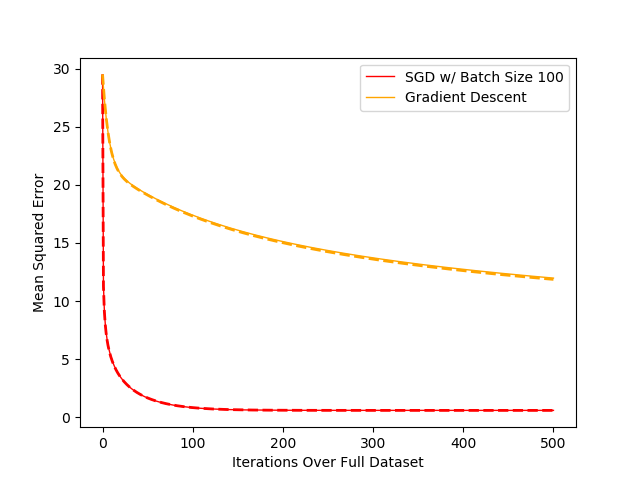
\includegraphics[width= 18cm]{img/problem_3/algo_comparison.png}
}
\caption{\label{fig:fig5}Comparison of gradient descent convergence with that of stochastic gradient descent with batch size of 100. The optimization was performed with $\tau = 0.001$ and $\lambda = 0.01$. Solid lines indicate mean squared error on the training data, and dashed lines indicate MSE on the test data.}
\end{figure}

\begin{figure}[h!]
\centerline{
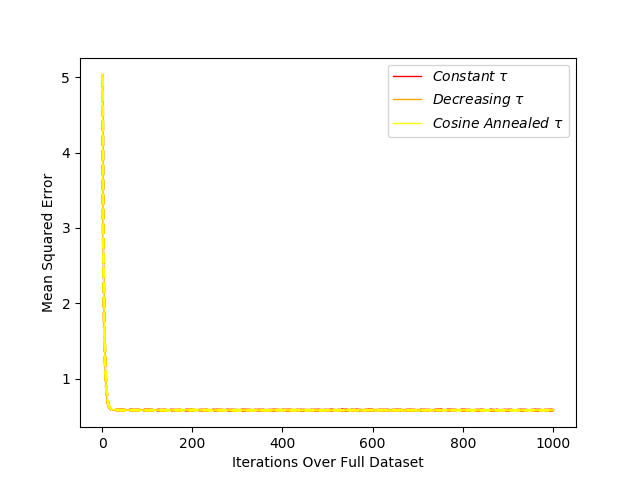
\includegraphics[width= 18cm]{img/problem_4/dynamic_time_stepping.png}
}
\caption{\label{fig:fig6}Comparison of stochastic gradient descent method applied to the ridge regression problem with various ridge coefficients. The batch size was fixed at 100, and the learning rate was fixed at $\tau=1e- 2$. Solid lines indicate mean squared error on the training data, and dashed lines indicate MSE on the test data.}
\end{figure}

and then the story continues.

\end{document}